%
% Documento: Fundamentação Teórica
%

\chapter{Fundamentação Teórica}
\label{chap:fundamentacaoTeorica}

A seguir ilustra-se a forma de incluir figuras, tabelas, equações, siglas e símbolos no documento, obtendo indexação automática em suas respectivas listas.
A numeração sequencial de figuras, tabelas e equações ocorre de modo automático.
Referências cruzadas são obtidas através dos comandos \verb#\label{}# e \verb#\ref{}#.
Por exemplo, não é necessário saber que o número deste capítulo é \ref{chap:fundamentacaoTeorica} para colocar o seu número no texto.
Isto facilita muito a inserção, remoção ou relocação de elementos numerados no texto (fato corriqueiro na escrita e correção de um documento acadêmico) sem a necessidade de renumerá-los todos.

\section{Figuras}
\label{sec:figuras}

Abaixo é apresentado um exemplo de figura.
A \autoref{fig:kdtree} aparece automaticamente na lista de figuras.
Para uso avançado de imagens no LATEX, recomenda-se a consulta de literatura especializada \cite{Goossens2007}.

\begin{figure}[!htb]
	\centering
	\caption{Exemplo da estrutura de uma árvore KD}
	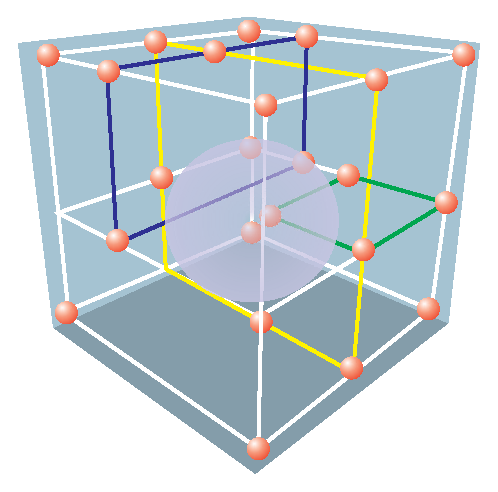
\includegraphics[width=0.3\textwidth]{./04-figuras/figkdtree}
	\fonte{\citeonline{CELSO2012}}
	\label{fig:kdtree}
\end{figure}

\section{Quadros e Tabelas}
\label{sec:tabelas}

Também é apresentado o exemplo do \autoref{qua:comparabd} e da \autoref{tab:correlacao}, que aparece automaticamente na lista de quadros e tabelas.
Informações sobre a construção de tabelas no LATEX podem ser encontradas na literatura especializada \cite{Lamport1986,Buerger1989,Kopka2003,Mittelbach2004}.

\begin{quadro}[!htb]
    \centering
    \caption{Hierarquia de restrições das questões.\label{qua:comparabd}}
    \begin{tabular}{|p{7cm}|p{7cm}|}
        \hline
        \textbf{BD Relacionais} & \textbf{BD Orientados a Objetos} \\
        \hline
        Os dados são passivos, ou seja, certas operações limitadas podem ser automaticamente acionadas quando os dados são usados. Os dados são ativos, ou seja, as solicitações fazem com que os objetos executem seus métodos. & Os processos que usam dados mudam constantemente. \\
        \hline
    \end{tabular}
    \fonte{\citeonline{carvalho:2001}}
\end{quadro}


Muitos confundem, mas existe diferença entre tabelas e quadros.
Um quadro é formado por linhas horizontais e verticais,
sendo, portanto ``fechado''. Normalmente é usado
para apresentar dados secundários. Nada impede, porém,
que um quadro apresente resultados da pesquisa.
Um quadro normalmente apresenta resultados
qualitativos (textos). O número do quadro e o título
vêm acima do quadro, e a fonte, deve vir abaixo.
Uma tabela é formada apenas por linhas verticais, sendo,
portanto ``aberta''. Normalmente é usada para
apresentar dados primários, e geralmente vem nos
“resultados” e na discussão do trabalho. Nada
impede, porém, que uma tabela seja usada no
referencial teórico de um trabalho. Uma tabela
normalmente apresenta resultados quantitativos
(números). O número da tabela e o título vêm
acima da tabela, e a fonte, deve vir abaixo, como
no quadro.

Exemplos de tabelas:

\begin{table}[!htb]
	\centering
	\begin{tabular}{cc}
		\hline
			x & y \\
		\hline
			1 & 2 \\
			3 & 4 \\
			5 & 6 \\
			7 & 8 \\
		\hline
	\end{tabular}
	\caption[Correlação de valores x e y]{Exemplo de uma tabela mostrando a correlação entre x e y.\label{tab:correlacao}}
%	\fonte{Autoria própria.}
\end{table}


\begin{table}[!htb]
    \centering
    \caption[Resultado dos testes]{Resultado dos testes.\label{tab:testes}}
    \begin{tabular}{rrrrr}
        \toprule
            & Valores 1 & Valores 2 & Valores 3 & Valores 4 \\
        \midrule
            Caso 1 & 0,86 & 0,77 & 0,81 & 163 \\
            Caso 2 & 0,19 & 0,74 & 0,25 & 180 \\
            Caso 3 & 1,00 & 1,00 & 1,00 & 170 \\
        \bottomrule
    \end{tabular}
\end{table}


\section{Equações}
\label{sec:equacoes}

A transformada de Laplace é dada na \autoref{eq:laplace}, enquanto a \autoref{eq:dft} apresenta a formulação da transformada discreta de Fourier bidimensional\footnote{Deve-se reparar na formatação esteticamente perfeita destas equações.}.

\begin{equation}
	X(s) = \int\limits_{t = -\infty}^{\infty} x(t) \, \text{e}^{-st} \, dt
	\label{eq:laplace}
\end{equation}

\begin{equation}
	F(u, v) = \sum_{m = 0}^{M - 1} \sum_{n = 0}^{N - 1} f(m, n) \exp \left[ -j 2 \pi \left( \frac{u m}{M} + \frac{v n}{N} \right) \right]
	\label{eq:dft}
\end{equation}

\section{Algoritmos}\label{sec:algoritmos}

Os algoritmos devem ser feitos segundo o modelo abaixo.
Para isso, utilizar o pacote {\ttfamily algorithm2e} no início do arquivo principal como neste exemplo.
O \autoref{alg:vertices} mostra um exemplo.

\begin{algorithm}
\caption{Algoritmo para remoção aleatória de vértices}
\KwIn{o número $n$ de vértices a remover, grafo original $G(V, E)$}
\KwOut{grafo reduzido $G'(V,E)$}
$removidos \leftarrow 0$ \\
\While {removidos $<$ n } {
	$v \leftarrow$ Random$(1, ..., k) \in V$ \\
		\For {$u \in adjacentes(v)$} {
			remove aresta (u, v)\\
			$removidos \leftarrow removidos + 1$\\
		}
		\If {há  componentes desconectados} {
			remove os componentes desconectados\\
		}
	}
\end{algorithm}

